\documentclass[10pt]{beamer}

\usepackage[utf8]{inputenc}
\usepackage{pgfpages}
\usepackage{dirtree}
\setbeamertemplate{note page}[plain]
\AtEndNote{\vfill \begin{center} mm:hh \end{center}}
\newcommand{\notedir}[1] {
  \note{\dirtree{#1}}}
\def \ion {$^{\circ}$ }
\usepackage{tcolorbox}
\usepackage{tikz}
\usepackage{tikz-3dplot}
\usetikzlibrary{intersections,calc,,angles,quotes,through}
\usepackage{amsmath}
\usepackage{graphicx}
\usepackage{cases}
\def \heart {\textcolor{blue}{$\heartsuit$} }
\def \C {\mathcal{C}}
\def \orthog {\underline{\perp}}
\def\arcos{\operatorname{arcos}}

\tcbset{%
	basic/.style={colframe=black,
		      colback=white,
		      top= 0mm,
		      bottom = 2mm,
		      boxsep=0mm
		      }
}
\tikzset{
    invisible/.style={opacity=0},
    visible on/.style={alt={#1{}{invisible}}},
    alt/.code args={<#1>#2#3}{%
      \alt<#1>{\pgfkeysalso{#2}}{\pgfkeysalso{#3}} % \pgfkeysalso doesn't change the path
    },
  }

    \def\enonce{ \frametitle{Exercice supplémentaire.}
	  %\renewcommand{\theenumi}{\alph{enumi})}
	  Soit un triangle $ABC$ et son cercle circonscrit $\C$. On note $t$ la tangente à
	  ce cercle passant par $A$ et $b$ la bissectrice de l’angle $\widehat{BAC}$. On note $B'$ et
	  $C'$ les images respectives de $B$ et $C$ par la symétrie orthogonale d’axe $b$.
	  Montrer que $B'C'$ est parallèle à $t$.
  }
  \def\hypotheses{ \underline{Hypothèses} 
		      \begin{enumerate}
		      \item $b$ bissectrice en $A$,
		      \item $B'$ symétrique de $B$ \\
			    $C'$ symétrique de $C$,
		      \item $t$ tangente en $A$,
		      \end{enumerate}
  }
  \def\these{  \underline{Thèse} \\
		      \smallskip
		      $B'C' \parallel t $.
}
    
\begin{document}  
    \beamertemplatenavigationsymbolsempty
    \setlength{\abovedisplayskip}{0pt}
    \setlength{\belowdisplayskip}{0pt}
    \frame{
	  
	 \enonce
	  \vfill
	  
	  \pause
	  % hypothèses et thèse
	  \begin{tcolorbox}[basic] 
	      \begin{columns}[t]
		 
		 \column{.5\textwidth}\centering
		      
		     \hypotheses

		  
		  \column{.5\textwidth}\centering
		      
		   \these
		
	      \end{columns}
	  \end{tcolorbox}
	  {\small Référence : LICOIS J-R., 2005. \textit{La géométrie élémentaire au fil de son histoire dans les programmes
			    français.} Ellipses, 134p.}
	\notedir{%
	.1 Énoncé.
	.2 Hypothèses (non visibles sur le dessin)..
	.2 Thèse..
	.2 Grand dessin.. 
	}
    }

    \frame{ 
	  % résolution ex1
	  \begin{columns}[t]
		\column{.5\textwidth}\centering 
		

			\underline{Dessin}\\
			
				  \begin{figure}[h]
				  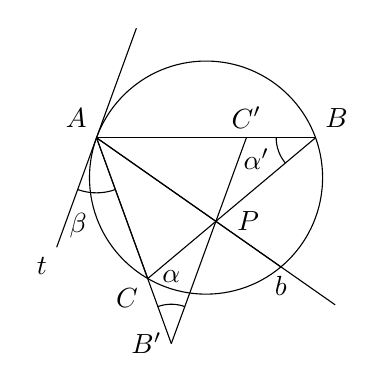
\begin{tikzpicture}[scale=0.74]
			          %projection ($(X)!(B')!(B)$)
			          %nommer chemin 'name path
			          %intersection \path [name intersections={of=d and gb,by=G}];
			          %animation  \draw[visible on=<1>] 
				  %           \draw[visible on=<{2,4}>]
				  %angle arc[radius = 6mm, start angle= 180, end angle= 225] node [below left,pos=0.3]{$\alpha$}
				  %angle \pic [draw, visible on=<2>, above left,"$\beta$", angle eccentricity=1.5] {angle = A'--A--B};
				  %perpendiculaire ($(A')!3cm!-90:(A)$)
				  
				  %CERCLE et triangle
				  \coordinate (O) at (0,0);
				  \coordinate[label=above right:$B$] (B) at (20:2);
				  \coordinate[label=below left:$C$] (C) at (-120:2);
				  \coordinate[label=above left:$A$] (A) at (160:2);
				  \draw[name path =cercle] (O) circle (2);
				  \draw (A) -- (B);
				  \draw (C) -- (A);
				  \draw[name path=BC] (B) -- (C); 				 
				  %Bissectrice b
				  \draw[] (A) -- +(-35:5) coordinate[](b');
				  \path[name path = b] (A) -- (b');
				  \path [name intersections={of=cercle and b,by=b}];
				  \coordinate[label=below:$b$]() at (b);
				  \draw (A) -- (b);
				  %C'
				  \path (C) -- +($2*(A)!(C)!(b)-2*(C)$) coordinate[label=above:$C'$](C'); 				  
				  %B'
				  \path (B) -- +($2*(A)!(B)!(b)-2*(B)$) coordinate[label=left:$B'$](B'); 
				  \draw[name path=B'C'] (B') -- (C');
				  \draw (A) -- (B');
				  %Tangente t
				  \draw (A) -- ($(A)!2cm!-90:(O)$)  coordinate[label=below left:$t$](t)-- ($(A)!2cm!90:(O)$);
				  %ANGLES
				  \pic [draw,"$\alpha$", angle eccentricity=1.7] {angle = C'--B'--A};
				  \pic [draw,"$\alpha'$", angle eccentricity=1.6] {angle = A--B--C};
				  \pic [draw,"$\beta$", angle eccentricity=1.6,left,angle radius=7mm] {angle = t--A--C};
				  %P
				  \path [name intersections={of= BC and B'C',by=P}];
				  \coordinate [label=right:$P$,xshift=1.5mm]() at (P);
				  \end{tikzpicture}				
				  \end{figure}
				  \vspace{-3mm}
				  \begin{tcolorbox}[basic] 
				      
				    \smallskip
				    \hypotheses
							      
				    \these
				    \end{tcolorbox}
		
		
		\column{.5\textwidth}\centering
		
		\underline{Résolution}\\ \flushleft
		
		\heart Deux $\Delta$ sont isométriques lorsqu'ils ont un angle de même mesure compris entre deux côtés de mêmes longueurs. \\ \medskip
		$\Delta ABP, \Delta AB'P$ isométriques car :
                
	$$	\begin{cases}
		 \widehat{CAP}=\widehat{PAB}, (\textcolor{blue}{1.})\\
		 |AB|=|AB'|, (\textcolor{blue}{2.})\\
                  [AP] \text{ en commun}. 
		\end{cases}\rightarrow \alpha = \alpha ' \smallskip
                $$
               \medskip
		 
		 \heart La mesure de l'angle tangentiel est égal à celle de l'angle inscrit interceptant le même arc. \\ \smallskip
		 $\beta = \alpha '$. \\ \medskip
		 $\rightarrow \alpha = \beta \rightarrow B'C' \parallel t$. \hfill $\qed$ \\ 

	   \end{columns}
  \notedir{%
	   .1 Prouver thèse.
	   .2 $B'C' \parallel t $.
	   .3 Élément de théorie.
	   .4 2 droites sont parallèles si deux angles correspondants qu'elles déterminent sont égaux..
	   .3 Résolution..
	   .4 $\Delta ABP, \Delta AB'P$ isométriques car.
	   .5 $\widehat{CAP}=\widehat{PAB}$ car $AP$ bissectrice..
	   .5 $|AB|=|AB'|$ car $B'$ est symétrique de $B$..
	   .5 Côté $[AP]$ en commun..
	   .4 $\Delta ABP, \Delta AB'P$ isométriques $\rightarrow \alpha = \alpha '$..
	   .4 Pour un même arc, angle tangentiel = angle inscrit..
	   .5 $\beta = \alpha '$..
	   .4 $\rightarrow \alpha = \beta$..
	   .5 $B'C'$ et $t$ parallèles car les deux angles correspondants sont égaux..
         }
         }
                    \frame{ 
	  \enonce

	  \vfill\center
	  \underline{Résumé}\\ \flushleft
          \begin{itemize}
	  \item  Montrer que 2 droites sont $\parallel$ = montrer que les angles alternes-internes sont égaux ?
          \item  Deux $\Delta$ sont isométriques lorsqu'ils ont un angle de même mesure compris entre deux côtés de mêmes longueurs.
            \item La mesure de l'angle tangentiel est égal à celle de l'angle inscrit interceptant le même arc.
          \end{itemize}
    }
    
	  
  
\end{document}

%%% Local Variables:
%%% mode: latex
%%% TeX-master: t
%%% End:
